%!TEX root = ../dissertation.tex
\begin{savequote}[75mm]
Nulla facilisi. In vel sem. Morbi id urna in diam dignissim feugiat. Proin molestie tortor eu velit. Aliquam erat volutpat. Nullam ultrices, diam tempus vulputate egestas, eros pede varius leo.
\qauthor{Quoteauthor Lastname}
\end{savequote}

\chapter{Experiment and results}

SCALETTA

* datasets
  * flickr
  * referit
* evaluation metric
* impl details
* model selection
* results
* qualitative results

\section{Datasets}
\label{sec:datasets}

In this section we describe Flickr30K and ReferIt, the two datasets
used for the experimental assessment. \todo{??? Furthermore, we
describe two other noteworthy and popular datasets available in
literature}

\subsection{Flickr30K}

Flickr30K Entities \todo{CITE: Flickr30K Entities} is a dataset built
on top of Flickr30K \todo{CITE: From image descriptions to visual
denotations: New similarity metrics for semantic inference over event
descriptions}. It is usually referred as Flickr30K or simply as Flickr
and, compared to the original Flickr30K dataset, it focuses on the
task of grounding textual mentions of entities in image by augmenting
data with extra annotations.

Annotations consists of cross-caption coreference chains linking
mentions of the same entities together with bounding boxes localizing
those entities in the image, and are collected throught a
crowdsourcing protocol. These annotations are highly structured and
vary in complexity from image to image, since images vary in the
numbers of clearly distinguishable entities they contain, and
sentences vary in the extent of their detail. Further, there are
ambiguities involved in identifying whether two mentions refer to the
same entity or set of entities, how many boxes (if any) these entities
require, and whether these boxes are of sufficiently high quality. To
tackle this problem, compounded by the unreliability of crowdsourced
judgments, they administer a pipeline of simple and atomic tasks which
can be grouped into two main stages: coreference resolution, or
forming coreference chains that refer to the same entities, and
bounding box annotation for the resulting chains. This workflow
provides two advantages: first, identifying coreferent mentions helps
reduce redundancy and save box-drawing effort; and second, coreference
annotation is intrinsically valuable. In
Fig.~\ref{fig:flickr30k-example}, taken from \todo{CITE: flickr30k
entitites} are shown the interfaces used to gather annotations with
respect to tasks described next.

\begin{figure}
  \centering
  \begin{subfigure}{.45\textwidth}
    \centering
    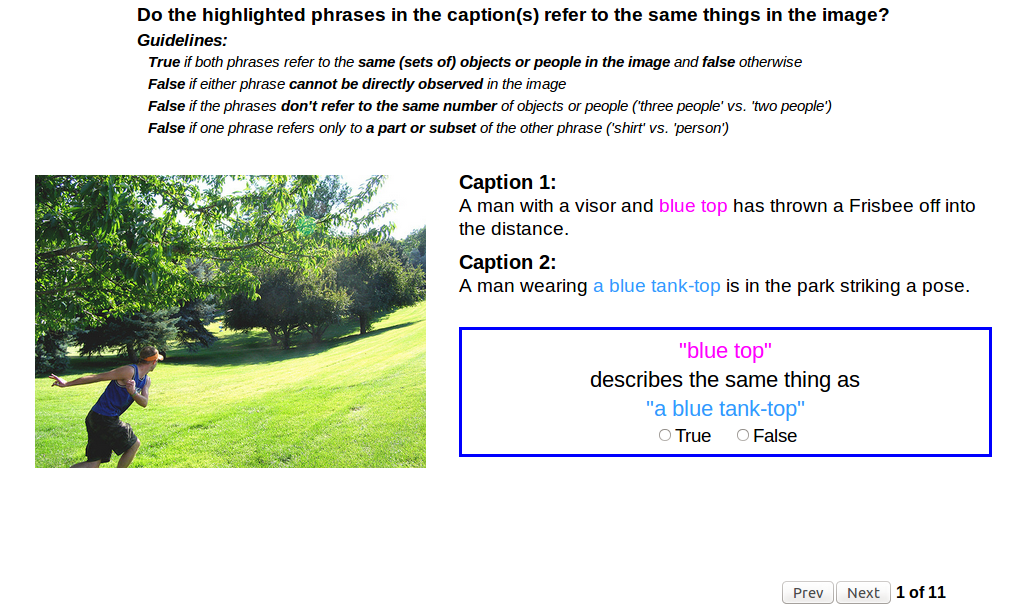
\includegraphics[width=.8\linewidth]{figures/flickr30k-example-coref-annotation.png}
    \caption{Binary coreference link interface}
    \label{fig:flickr30k-example-coref-annotation}
  \end{subfigure}
  \begin{subfigure}{.45\textwidth}
    \centering
    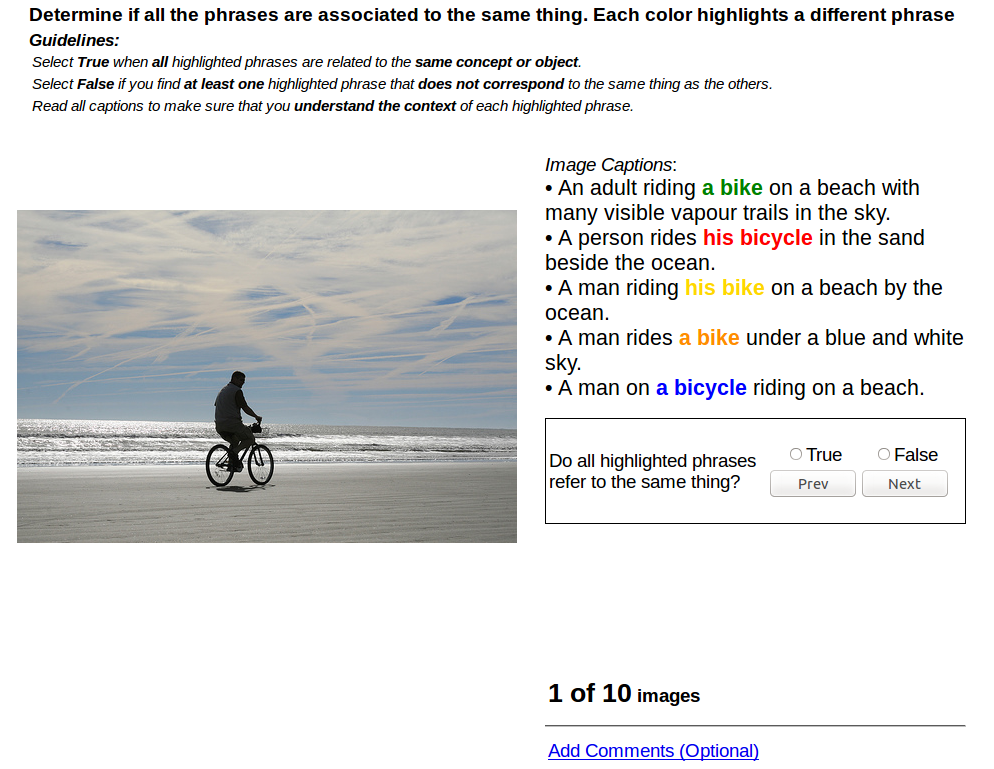
\includegraphics[width=.8\linewidth]{figures/flickr30k-example-coref-verification.png}
    \caption{Coreference chain verification interface}
    \label{fig:flickr30k-example-coref-verification}
  \end{subfigure}
  \begin{subfigure}{.45\textwidth}
    \centering
    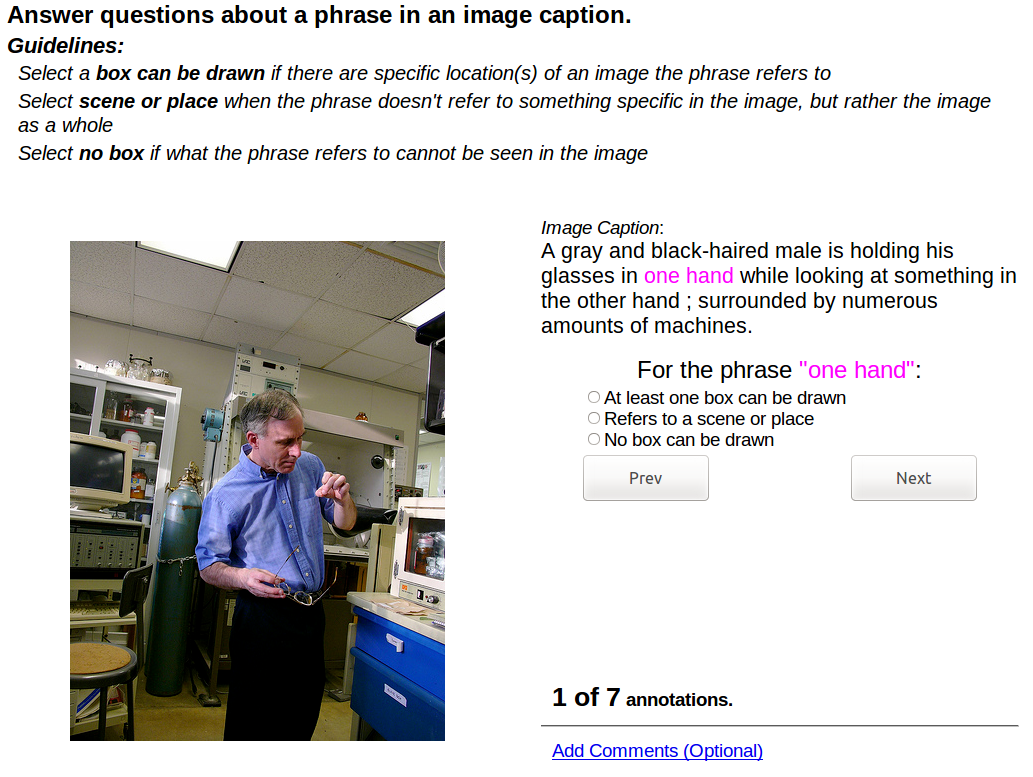
\includegraphics[width=.8\linewidth]{figures/flickr30k-example-box-requirement.png}
    \caption{Box requirement interface}
    \label{fig:flickr30k-example-box-requirement}
  \end{subfigure}
  \begin{subfigure}{.45\textwidth}
    \centering
    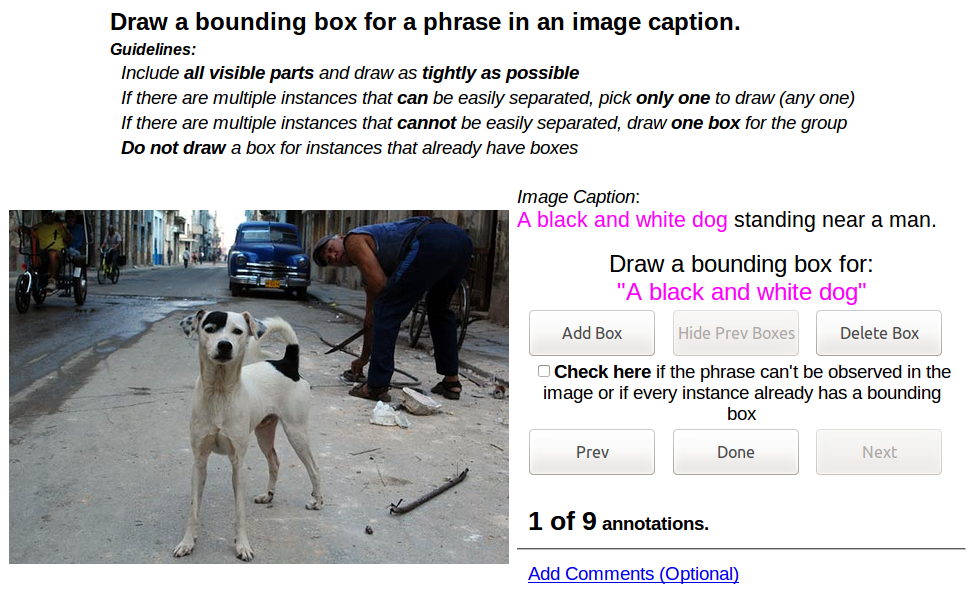
\includegraphics[width=.8\linewidth]{figures/flickr30k-example-box-drawing.png}
    \caption{Box drawing interface}
    \label{fig:flickr30k-example-box-drawing}
  \end{subfigure}
  \begin{subfigure}{.45\textwidth}
    \centering
    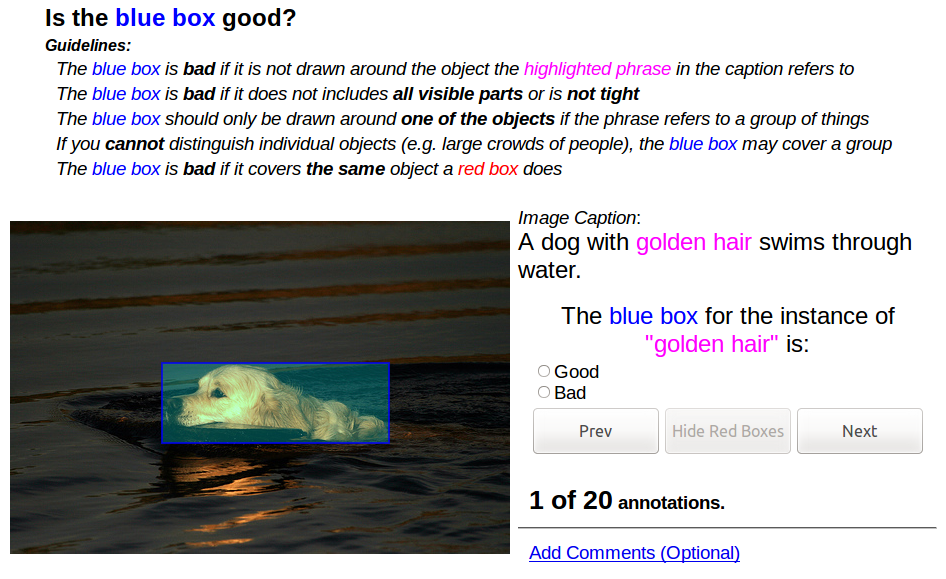
\includegraphics[width=.8\linewidth]{figures/flickr30k-example-box-quality.png}
    \caption{Box quality interface}
    \label{fig:flickr30k-example-box-quality}
  \end{subfigure}
  \begin{subfigure}{.45\textwidth}
    \centering
    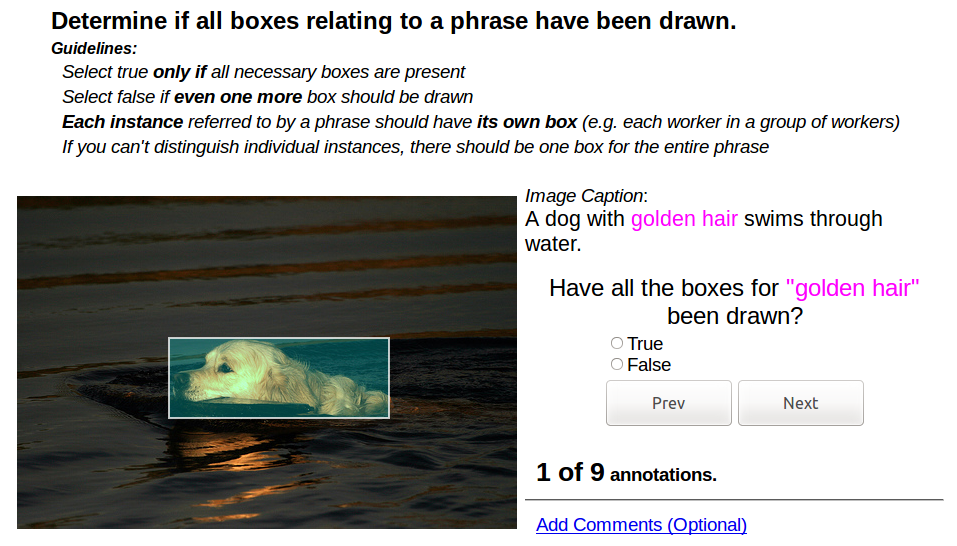
\includegraphics[width=.8\linewidth]{figures/flickr30k-example-box-coverage.png}
    \caption{Box coverage interface}
    \label{fig:flickr30k-example-box-coverage}
  \end{subfigure}
  \caption{Examples of the interfaces used in TODO CITE FLICKR annotation system.}
  \label{fig:flickr30k-example}
\end{figure}

The coreference resolution task is solved by first chunking
information given in Flickr captions to identify potential entity
mentions. Each chunk, i.e., noun phrase (NP), is a potential entity
mention. For example, the frase ``A man in an orange hat'' is chunked
in two noun phrases, namely ``A man'' and ``an orange hat'', which are
the two mentions. Given $M$ a document containing noun phrases
originated from captions of an image, a worker is required to specify
whether two given mentions $m$ and $m'$ refer to the same entity. If
the answer is positive, a link between the two mentions is addded,
creating a coreference chain. Tipically, this would require $O(|M|^2)$
which is the cost of all pairwise links. But since $M$ usually
contains multiple mentions that refer to the same set of entities, the
number of coreference chains is bounded by a number much smaller than
$|M|$, on average. Also, the bound is lowered by making two assumptions.
First, they assume that mentions from the same captions cannot be
coreferent; second, they categorize each mention into eight
coarse-grained types using manually constructed dictionaries (people,
body parts, animals, clothing/color, instruments, vehicles, scene, and
other), and assume mentions belonging to different categories cannot
be coreferent. The goodnees of the strategy is empirically shown by a
small-scale test on 200 images and the coreference chains are verified
by another task which asks to a worker whether given mentions in
coreference chain refer to the same entity. Their results shows that
only $9.8\%$ of all coreference chains are not correct.

Bounding box annotation is carried out with a workflow composed by
four tasks administered to workers, namely: box requirement, box
drawing, box quality and box coverage. In box requirement, a worker
needs to specify, whether at least one bounding box can be drawn in
image for given mention. If the response is negative, the mention
leaves the workflow, otherwise it goes throught the box drawing stage.
Here, a worker should draw a box as tight as possible around the
mentioned entity. The main source of difficulty in this stage is due
to mentions that refer to multiple entities. If a box is drawn, then
the mention-box pair proceeds to box quality stage. At this point,
drawn box is evaluated in terms of redundancy (are there any box that
already covers the same entity?), accuracy (is the box tight around
the entity?), distinctiveness (can a box be drawn for single entity
instead of covering multiple elements?). If the answer is positive,
the example goes to the last stage. In box coverage, workers decide
whether all required boxes are present in image. 

During the annotation process, workers are subjected to quality
control process. Workers must pass a test before being allowed to
annotate dataset examples. Also, during the annotation process,
workers are asked some verification questions (question with known
answer, written by authors).

In the end, Flicker30K Entities is made up of 32K images, 159K
sentences, 275K bounding boxes, and 360K noun phrases where each image
is associated with five sentences with a variable number of noun
phrases, and each noun phrase is associated with a set of bounding
boxes ground truth coordinates. 

\subsubsection{Data Representation}
\label{subsec:flickr30k-data-representation}

Technically speaking, in Flickr30K Entities each example is composed
by information contained in three different files linked together by
means of an identifier $id$. Those files represent image, sentence
annotations and image annotations information. The image file is
simply a JPG file, while the sentence annotations file is a textual
document containing five captions. Each caption is chunked into a
variable number of noun phrases and each noun phrase can be linked to
a bounding box contained in the third file. The image annotation file
is an XML file with an array of objects. Every object has one or more
name, that can be used to reconstruct which noun phrase is linked to
the bounding box, and four coordinates $x_{min}, y_{min}, x_{max},
y_{max}$ if it is a visual element, none otherwise. The structure is
visually explained in
Fig.~\ref{fig:flickr30k-technical-data-representation}.

\begin{figure}
  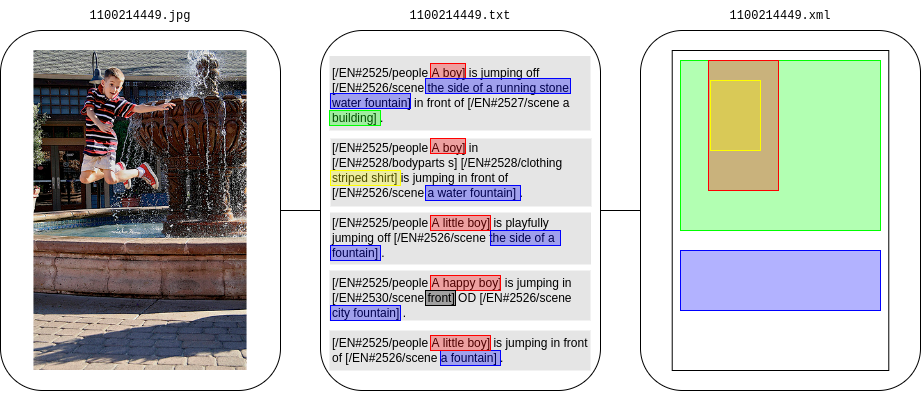
\includegraphics[width=\textwidth]{figures/flickr30k-document-specification.png}
  \caption[TODO]{TODO: rappresentare i tre file e collegare gli ID con i colori evidenziano l'esempio, le query e le noun phrase per query. Aggiornare immagine con i nuovi fix}
  \label{fig:flickr30k-technical-data-representation}
\end{figure}

Those data ara available online in two parts: images and can be
downloaded by compiling a registration form,
\footnote{\href{http://shannon.cs.illinois.edu/DenotationGraph/}{http://shannon.cs.illinois.edu/DenotationGraph/}}
while annotations, instead, do not requires a sign up: data can be
downloaded from B. A. Plummer repository on GitHub.
\footnote{\href{https://github.com/BryanPlummer/flickr30k\_entities}{https://github.com/BryanPlummer/flickr30k\_entities}}
Within the repository, authors have made available predefined
training, validation and test split that we use in our work, following
current literature.

\subsection{ReferIt}

ReferIt \todo{CITE: referit} is another popular dataset. The reason
that led to developing this dataset is to study how people refer to
objects in complex photographs of a real-world cluttered scenese.
Thus, the focus is on referring expression grounding task. However,
due to the heterogeneity of data, it can be employed also in phrase
grounding.

ReferIt contains very challenging examples from phrase groudning point
of view, because the dataset is collected entirely in an unsupervised
context by crowd throught a game. Examples vary from ``a man'' and
``the person in red'' to ``buildings'' or more degenrative ones like
``i don't think that was trash, lol. anyway, wall just above heads''.
In ReferIt many phrases uses spatial relations among objects, such as
``building on right behind guys'' or ``window top 2nd left''.

Referring expressions are collected through \textit{ReferItGame},
which is a two-player online game. The game is the key point of the
whole dataset, because it allow to collect large-scale dataset
containing natural language expressions referring to objects in
photographs of real world scenes in an inexpansive way.

The game is a simple two player game where players alternate between
generating expressions referring to objects in images of natural
scenes, and clicking on the locations of described objects.
Fig.~\ref{fig:referitgame-example}, from \todo{CITE: referit paper}
shows an example of the game. The game play is straightforward: an
image with an object outlined in red and a text box is show to Player
1. Player 2 instead receives, the same image and the referring
expression written by Player 1 and must click on the location of the
described object (note, Player 2 does not see the object
segmentation). If Player 2 clicks on the correct object, then both
players receive game points and the Player 1 and Player 2 roles swap
for the next image. If Player 2 does not click on the correct object
then no points are received and the players remain in their current
roles. When there are no players available for a player vs player
match, then a canned match is started where the missing player is
replaced by a CPU palyer. In this way, by design the referring
expression are provided and also verificated. 

\begin{figure}
  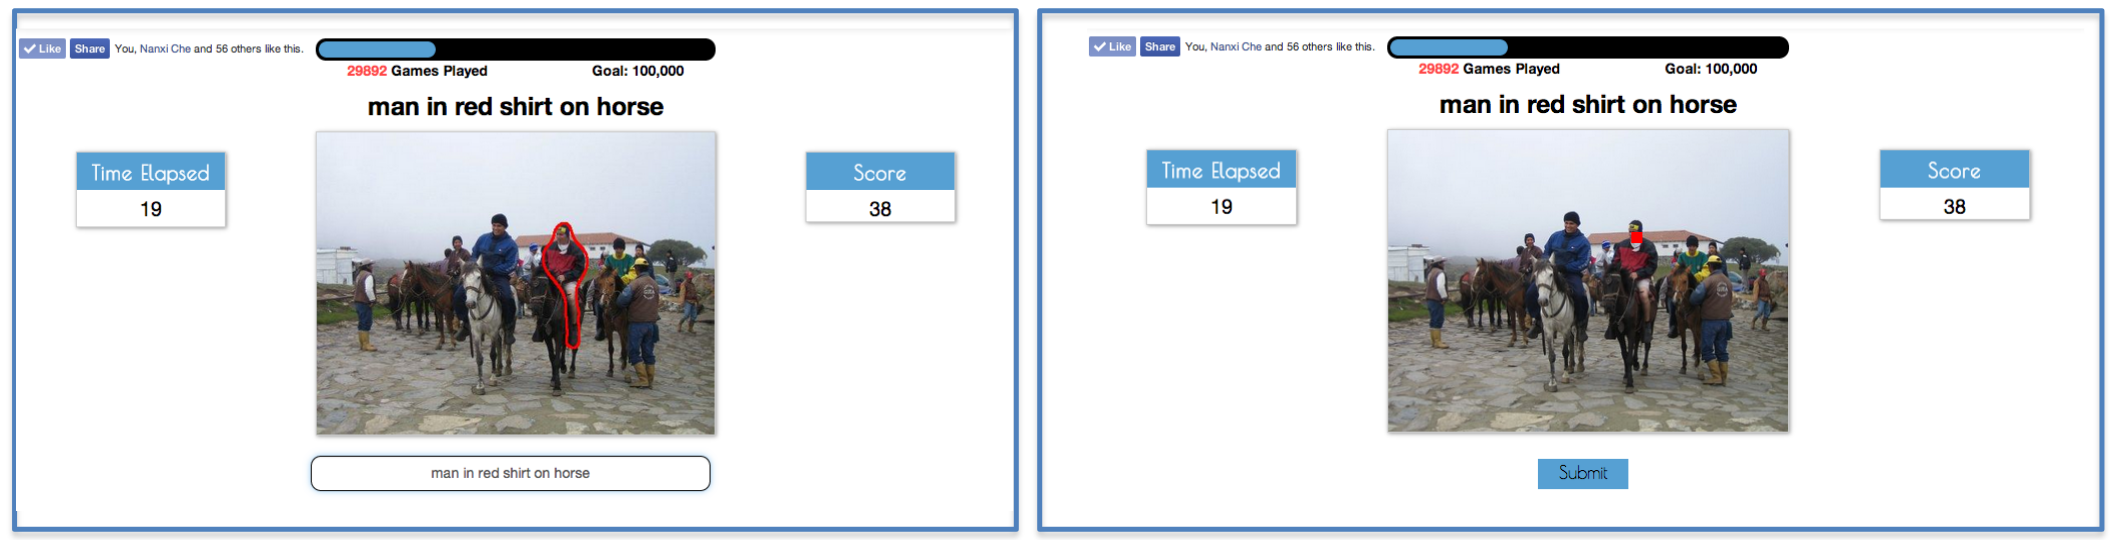
\includegraphics[width=\textwidth]{figures/referitgame-example.png}
  \caption[ReferIt Game Example.]{An example game from \todo{CITE:
  referit}. Player 1 \textit{(left)} sees an image with an object
  outlined in red (the man) and provides a referring expression for
  the object (``man in red shirt on horse''). Player 2
  \textit{(right)} sees the image and the expression from Player 1 and
  must localize the correct object by clicking on it (click indicated
  by the red square). Elapsed time and current scores are also
  provided.}
  \label{fig:referitgame-example}
\end{figure}

\subsubsection{Data Representation}
\label{subsec:referit-data-representation}

All ReferIt data is available online and instructions are provided at
Licheng Yu's GitHub
repository.\footnote{\href{https://github.com/lichengunc/refer}{https://github.com/lichengunc/refer}}
Images are stored in JPG files, while annotations are described
throught two structured file. One is a JSON file containing the
bounding box annotations along with a list of images and their $id$,
the other is a PICKLE
file\footnote{\href{https://docs.python.org/3/library/pickle.html}{https://docs.python.org/3/library/pickle.html}}
containing a serialized Python object that represents sentence
annotations. The Fig.~\ref{fig:referit-technical-data-representation} depict
described structure.

\begin{figure}
  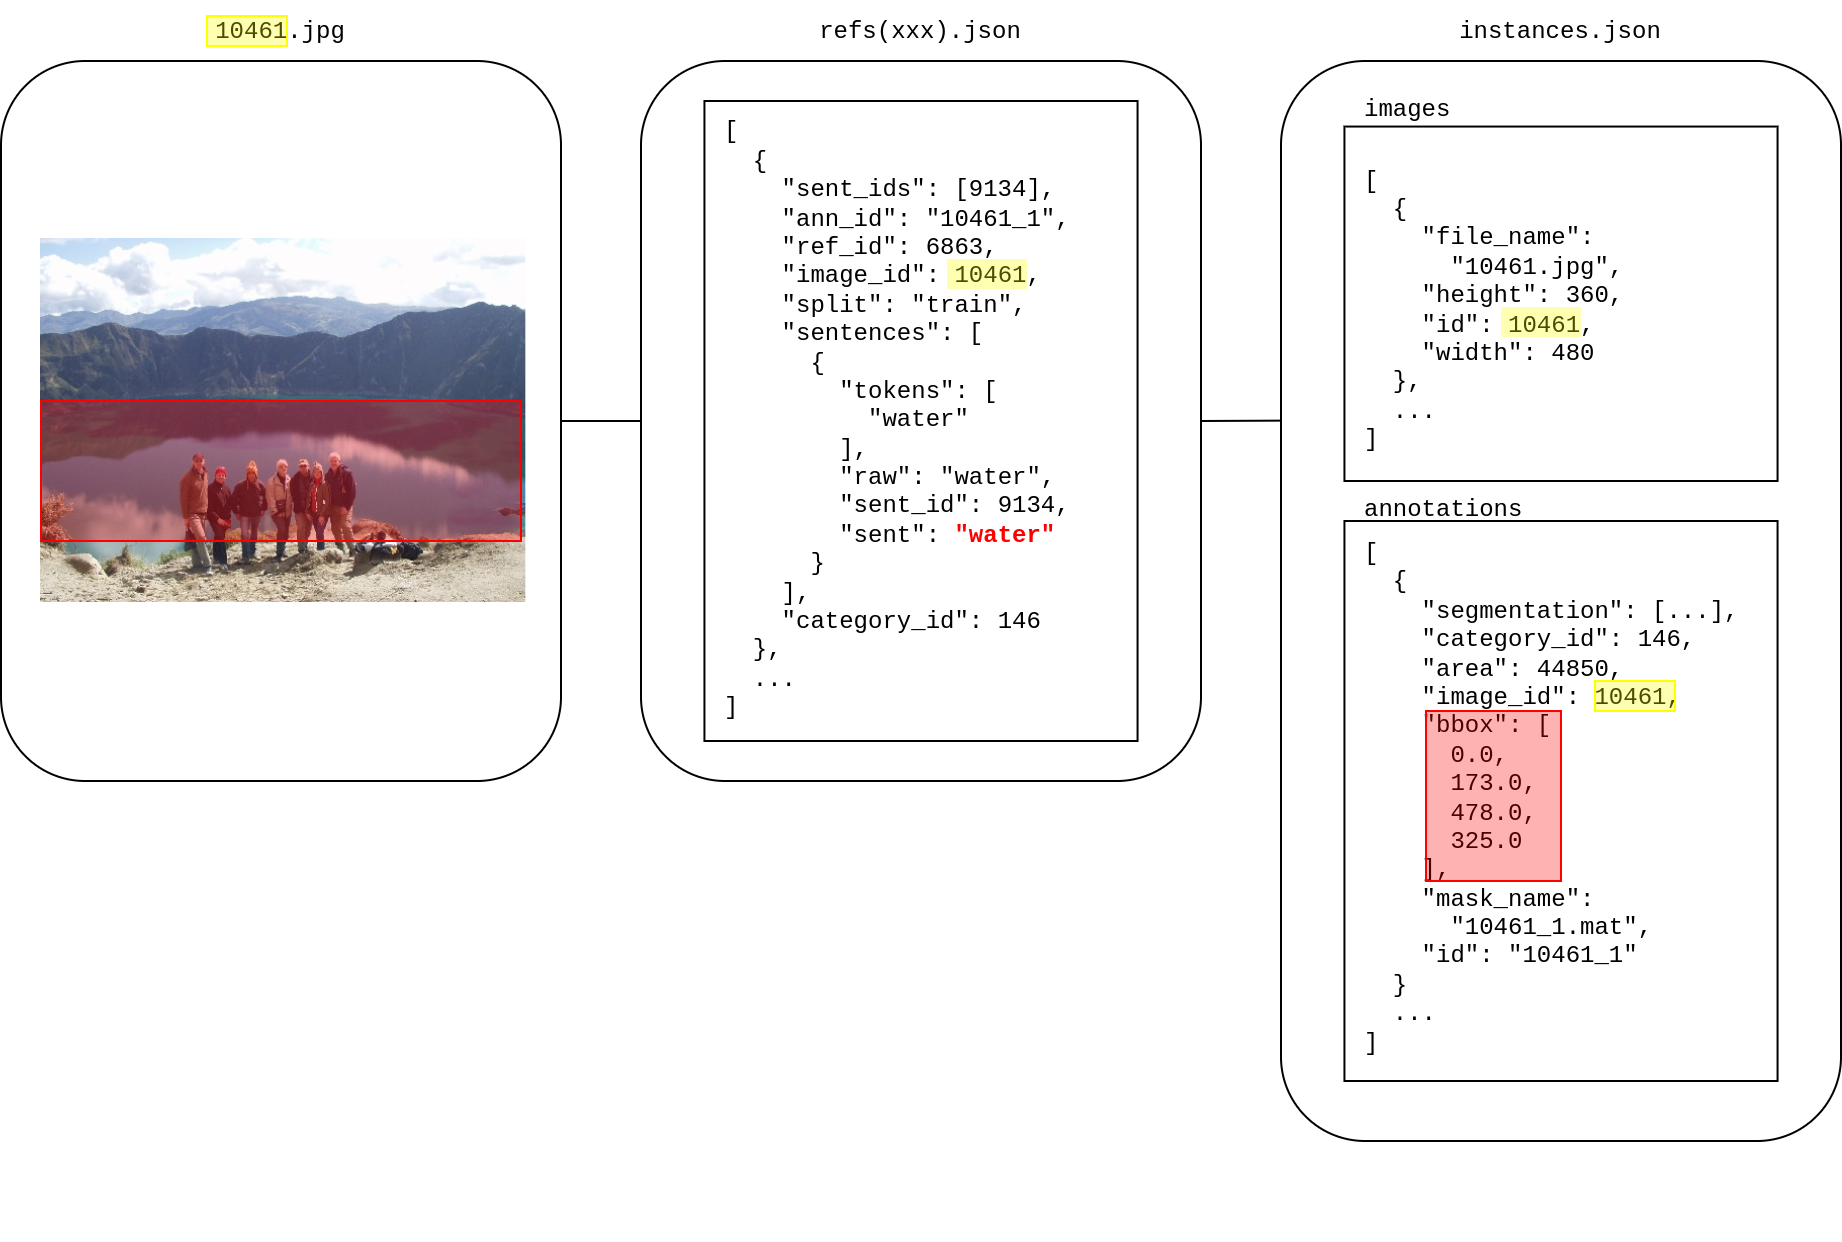
\includegraphics[width=\textwidth]{figures/referit-document-specification.png}
  \caption[TODO]{TODO: desc}
  \label{fig:referit-technical-data-representation}
\end{figure}

\section{Data analysis}

 \todo{prima o dopo data preprocessing??}

\section{Data preprocessing}

It is well known that data preparation and filtering steps take
considerable amount of processing time in machine learning problems
\cite{kotsiantis2006data}. Most of the time, data we collect or borrow
are biased, flowed, redundant, maybe irrelevant and sometimes
corrupted or missing. For the development of an accurate and general
model, the representation and quality of the instance data must be
maximized by working on task like cleaning, normalization,
transformation, feature extraction and selection. Fortunately, we do
not work with row data: due to the large adoption of datasets
described in Sec.~\ref{sec:datasets}, provided data are already
preprocessed in a grossly way.

However, in the next section we describe our preprocessing pipeline,
focusing on data representation which can be confusing due to the
etherogeneity of representations.

\subsection{Data preparation}

Given data as specified in
Sec.~\ref{subsec:flickr30k-data-representation} and
\ref{subsec:referit-data-representation} both for Flickr30K and
ReferIt, we create a single and unified interface for data where
information are represented homogeneously. Then we augment data, and
we fix some problems coming from dataset.

TODO: riassumere pipeline, funzioni extract ingo, remove\_queries\_and\_new\_var

TOOD: discutere operations on single element e varie trasformazioni

TODO: argomantere il padding e la creazione del batch

TODO: aggiungere descrizione "formale", elencando le chiavi del dizionario del batch

TODO \todo{AGGIUNGERE in extract inf/remove queries (prima parte)} Following all works in literature, if a noun
phrase corresponds to multiple ground truth bounding boxes, we merge
the boxes and use their union region as its ground truth. On the
contrary, if a noun phrase has no associated bounding box, we remove
it from the dataset. We use the standard split for training,
validation, and test set as defined in  \todo{CITE: Flickr30K
Entities}, consisting of 30K, 1K, and 1K images, respectively.